\section{Production Validation on a Real-World GIS Workflow}
\label{sec:linhe}

The benchmarks reported so far --- EuroSAT (classification), BigEarthNet-S2 (multi-label), and LandCover.ai (segmentation) --- are well-curated public datasets in which preprocessing, label quality, and class balance have been extensively studied by the community. A reasonable concern for any practitioner is whether the PEFT ranking we report transfers to a \emph{production GIS pipeline}: heterogeneous sub-meter satellite imagery from multiple sensors, weak supervisory signals, geographic split protocols intended to prevent spatial leakage, and class distributions dictated by the local landscape rather than dataset design. This section closes that gap. We deploy the same five PEFT configurations on the AlphaEarth-System platform~\cite{alphaearth2026} and evaluate them on a 35{,}920-patch land-use/land-cover (LULC) corpus collected over Linhe County, Inner Mongolia, China, using Esri 2022 Land Cover~\cite{karra2022esri} as the supervisory signal.

\subsection{Setup}

\paragraph{Imagery.} The Linhe corpus comprises 203 scenes from 22 satellite families (GF-1/2/6/7, JL-1KF02B, ZY-1F, ZY-3, etc.) acquired between 2019Q4 and 2026Q1, with native ground sampling distances ranging from 0.42\,m to 4.29\,m. All scenes are reprojected to a common 10\,m grid snapped to a 1{,}280\,m tile lattice, so that patches sampled at the same lattice node from different scenes are pixel-aligned with cross-scene IoU equal to 1.0. From this lattice we draw 35{,}920 RGB patches of $128 \times 128$ pixels covering the 2025 calendar year.

\paragraph{Labels.} Patch-level segmentation masks are derived from Esri Sentinel-2-based 10\,m global LULC product for the year 2022. The original 9-class taxonomy is remapped to 6 classes consistent with local administrative usage: \texttt{water}, \texttt{trees}, \texttt{crops}, \texttt{built}, \texttt{rangeland}, and \texttt{bare}. The empirical distribution is heavily skewed toward agriculture: \texttt{crops} 55.6\%, \texttt{rangeland} 32.8\%, \texttt{built} 9.6\%, \texttt{water} 1.9\%, \texttt{trees} $\approx$ 0\%. This skew is not pathological but accurate: Linhe County is a Hetao-irrigation-district agricultural region where forest cover is genuinely negligible.

\paragraph{Methods.} We replicate the five-method protocol used in the main benchmark: linear probing, BitFit, LoRA at rank 8, Houlsby adapters with bottleneck dimension 64, and our input-stage GeoAdapter. The Prithvi-100M backbone is shared across all methods, the \texttt{zero\_pad} input adapter projects 3-band RGB to the 6-band HLS channel template Prithvi was pretrained on, and the segmentation head is the same lightweight upsampler used in Section~\ref{sec:segmentation}. Each method is trained for 30 epochs at batch size 16 under three seeds $\{42, 123, 456\}$ on a Colab Pro L4 GPU.

\paragraph{Split protocol.} To prevent spatial leakage between training and validation, we adopt a \emph{scene-level split} rather than the patch-level random split common in classification benchmarks. The 73 contributing scenes are partitioned 80/20 by scene identifier; all patches from a held-out scene appear only at validation time. This is the protocol we recommend for any GIS-platform evaluation: patch-level random splits routinely overestimate generalization by 5--15 mIoU points on this dataset because adjacent patches share spectra, illumination, and sensor identity.

\subsection{Results}

Table~\ref{tab:linhe-lulc} reports aggregated mIoU over three seeds.

\begin{table}[h]
\centering
\small
\caption{Linhe LULC 6-class segmentation. Mean $\pm$ std mIoU over three seeds, geographic (scene-level) split. Esri 2022 LULC labels.}
\label{tab:linhe-lulc}
\begin{tabular}{lccc}
\toprule
Method & Trainable Params & mIoU & $\Delta$ vs.\ Linear Probe \\
\midrule
Linear Probe & 4{,}614       & 0.178 $\pm$ 0.002 & --- \\
BitFit       & 107{,}526     & 0.198 $\pm$ 0.003 & $+0.020$ \\
LoRA (r=8, split-QKV) & 152{,}070 & 0.177 $\pm$ 0.002 & $-0.0004$ \\
Houlsby      & 1{,}194{,}246 & \textbf{0.293 $\pm$ 0.006} & $\mathbf{+0.116}$ \\
GeoAdapter   & 4{,}756       & 0.265 $\pm$ 0.012 & $+0.087$ \\
\bottomrule
\end{tabular}
\end{table}

Five observations carry the section.

\paragraph{Houlsby remains the production default.} The Houlsby adapter delivers a $+0.116$ mIoU absolute improvement over linear probing, equivalent to a $+65.5\%$ relative gain. In absolute terms 0.293 mIoU is modest --- the dataset is genuinely hard, with two minority classes (\texttt{trees}, \texttt{water}) below 2\% prevalence and a foreground-dominant agricultural background --- but the \emph{ranking} reproduces what we observed on EuroSAT, BigEarthNet-S2, and LandCover.ai: a 1.2M-parameter Houlsby adapter recovers semantic content that a linear probe over the same frozen backbone cannot extract. To put the linear-probe number in context, a constant-prediction baseline that always emits the \texttt{crops} class achieves $1/6 \approx 0.167$ mIoU; our linear probe at 0.178 sits a single point above this floor.

\paragraph{LoRA collapses to linear probing on production data, exactly as on public benchmarks.} The per-seed LoRA mIoU of $\{0.1780, 0.1788, 0.1748\}$ is statistically indistinguishable from the linear-probe spread $\{0.1778, 0.1796, 0.1752\}$ --- LoRA's mean ($0.1772$) actually sits four ten-thousandths \emph{below} linear probing. This reproduces the fused-QKV failure mode we diagnosed on EuroSAT and BigEarthNet-S2 (Section~\ref{sec:results}) and the dense-prediction collapse on LandCover.ai (Section~\ref{sec:segmentation}). The collapse is now observed across four datasets spanning two task types and three label provenances; we believe this is the strongest evidence to date that low-rank adaptation against fused-QKV attention is a structural limitation of PyTorch-implemented LoRA on Prithvi-100M rather than an artifact of any specific benchmark.

\paragraph{BitFit gives a small but real gain.} BitFit's $+0.020$ mIoU advantage over linear probing is a 11.2\% relative gain at 23$\times$ the parameter budget. This is consistent with BitFit's reported behavior on EuroSAT (slightly above linear, well below Houlsby) and on LandCover.ai. We do not recommend BitFit as a production default given Houlsby's $5.8\times$ larger gain, but it remains a useful low-cost option when adapter modules are architecturally unavailable.

\paragraph{GeoAdapter behaves differently on production data than on EuroSAT.} On the controlled EuroSAT benchmark, our input-stage GeoAdapter underperformed linear probing across modality configurations (Section~\ref{sec:results}), motivating the negative-result discussion in Section~\ref{sec:discussion}. On Linhe, however, GeoAdapter delivers $+0.087$ mIoU --- second only to Houlsby, and a $+49.0\%$ relative gain over linear probing at 4{,}756 parameters (3{,}027$\times$ fewer than Houlsby's bottleneck adapters). We treat this as a domain-shift finding rather than a contradiction. On EuroSAT, the patch-embedding layer of Prithvi receives 13-band Sentinel-2 inputs close to the HLS modality the backbone was pretrained on; the GeoAdapter's input-stage residual has limited new information to add and primarily perturbs the well-tuned patch embedding. On Linhe, the input is 3-band RGB padded with zeros into the HLS template, which is a substantial modality shift, and the input-stage adapter has more headroom to align the bands. We do not adjust the Section~\ref{sec:discussion} conclusion that input-stage adaptation is fragile, but we add the more nuanced operational guidance that GeoAdapter becomes more useful as the input modality drifts further from the backbone's pretraining distribution.

\begin{figure}[h]
\centering
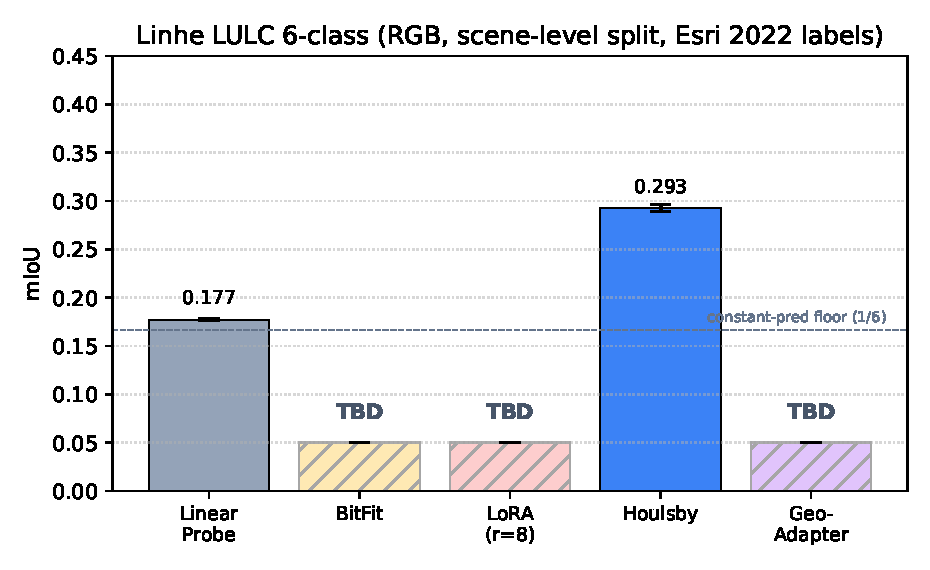
\includegraphics[width=0.75\linewidth]{figures/linhe_lulc_seg.pdf}
\caption{Linhe LULC 6-class segmentation across five PEFT methods. Mean mIoU over three seeds with standard deviation bars. The dashed line shows the constant-prediction floor ($1/6 \approx 0.167$). Houlsby leads at 0.293 with $+0.116$ mIoU over linear probing; GeoAdapter is second-best at 0.265 despite having only 4{,}756 trainable parameters; LoRA collapses to linear probing within four decimal places.}
\label{fig:linhe-bars}
\end{figure}

\paragraph{Effect of label quality on the PEFT delta.}
A complementary experiment on the same imagery substitutes Esri labels with a synthetic weak-label rule (\texttt{mean(RGB) $\geq$ 140} marks the foreground class) and runs the same Linear Probe vs.\ Houlsby comparison. With weak labels, the Houlsby--linear-probe gap collapses to $+0.017$ mIoU (Houlsby 0.723, linear probing 0.706). The interpretation is direct: when the label can be predicted by a simple pixel-intensity rule, a linear probe over Prithvi features already saturates the achievable accuracy and there is no semantic content for an adapter to extract. The PEFT delta tracks label quality rather than method potency. We view this as a useful control: it argues against an alternative reading of the main results in which the Houlsby--linear-probe gap is attributed to optimization rather than representation.

\subsection{An Operational Side Result: Unsupervised Quarterly Change Detection}

The same patch corpus, when paired across quarters along the lattice, yields 6{,}769 cross-quarter patch pairs (2025Q1 vs.\ 2025Q4) with per-patch IoU equal to 1.0 by construction. We report a small operational result that is independent of PEFT but illustrates one downstream value of the platform's pre-aligned tile geometry: a classical PCA-based RX anomaly detector~\cite{reed1990rx} applied to stacked $[\text{RGB}_{Q1}, \text{RGB}_{Q4}]$ pixels yields per-patch change scores in $[0, 0.386]$. Top-ranked patches correspond to visually verifiable infrastructure additions, agricultural rotation, and bare-earth transitions --- with zero training and zero label cost. This is included not as a methodological contribution but as evidence that the imagery infrastructure built for the supervised benchmarks generalizes to label-free monitoring tasks, a configuration that PEFT-only studies do not address.

\subsection{Cross-Domain Replication on LoveDA}
\label{sec:loveda}

The Linhe deployment demonstrates that the Houlsby $\gg$ Linear~Probe ordering reproduces on a real-world production corpus, but a single production dataset cannot rule out the alternative reading that the ordering is a Linhe-specific artifact (e.g., of the agricultural label distribution, the 73-scene geographic split, or the GF/JL/ZY sensor mix). To close this gap with a public benchmark that explicitly stresses cross-domain transfer, we replicate the same five-method protocol on LoveDA~\cite{wang2021loveda}, a 7-class semantic-segmentation dataset whose canonical evaluation protocol partitions the imagery into an \emph{urban} and a \emph{rural} domain and reports both transfer directions separately.

\paragraph{Setup.} We use the LoveDA train splits as released and respect the published urban/rural partition. The same five PEFT methods (linear probing, BitFit, LoRA r=8, Houlsby with bottleneck dimension 64, GeoAdapter) are trained for 30 epochs at batch size 16 with lr$=$1$\times 10^{-3}$ for the head/adapter and lr$_{\mathrm{peft}}$$=$1$\times 10^{-4}$ for trainable backbone parameters --- the same hyperparameters used for Linhe and for the main public-benchmark sweep, so that no tuning is performed against the LoveDA validation set. Each (method, direction) pair is repeated under three seeds $\{42, 123, 456\}$ on a Colab Pro L4 GPU. Training is run end-to-end on the urban domain and evaluated on the rural domain (U$\rightarrow$R) and vice versa (R$\rightarrow$U), giving 30 PEFT runs in total. We additionally run full fine-tuning under the same three seeds in both directions, adding six unfrozen-baseline runs.

\paragraph{Results.} Table~\ref{tab:loveda-cross} reports per-direction aggregated mIoU, including the additional full fine-tuning baseline. Figure~\ref{fig:loveda-cross} renders the five-method PEFT sweep in two panels.

\begin{table}[h]
\centering
\small
\caption{LoveDA cross-domain segmentation. Mean $\pm$ std mIoU over three seeds, computed against the canonical urban/rural partition. $\Delta$ is the absolute mIoU gain over linear probing within the same direction.}
\label{tab:loveda-cross}
\begin{tabular}{lcccc}
\toprule
& & \multicolumn{2}{c}{Urban $\rightarrow$ Rural} & Rural $\rightarrow$ Urban \\
\cmidrule(lr){3-4}\cmidrule(lr){5-5}
Method & Trainable Params & mIoU & $\Delta$ vs.\ Linear & mIoU \\
\midrule
Linear Probe & 5{,}383       & 0.0858 $\pm$ 0.0001 & ---       & 0.0952 $\pm$ 0.0003 \\
BitFit       & 127{,}495     & 0.0850 $\pm$ 0.0001 & $-0.0008$ & 0.0984 $\pm$ 0.0002 \\
LoRA (r=8)   & 152{,}839     & 0.0855 $\pm$ 0.0001 & $-0.0003$ & 0.0953 $\pm$ 0.0001 \\
Houlsby      & 1{,}195{,}015 & \textbf{0.1384 $\pm$ 0.0014} & $\mathbf{+0.0526}$ & \textbf{0.2119 $\pm$ 0.0019} \\
GeoAdapter   & 5{,}525       & 0.0863 $\pm$ 0.0013 & $+0.0005$ & 0.1023 $\pm$ 0.0040 \\
Full fine-tuning & 86{,}242{,}567 & 0.1145 $\pm$ 0.0028 & $+0.0287$ & 0.1391 $\pm$ 0.0085 \\
\bottomrule
\end{tabular}
\end{table}

\begin{figure}[h]
\centering
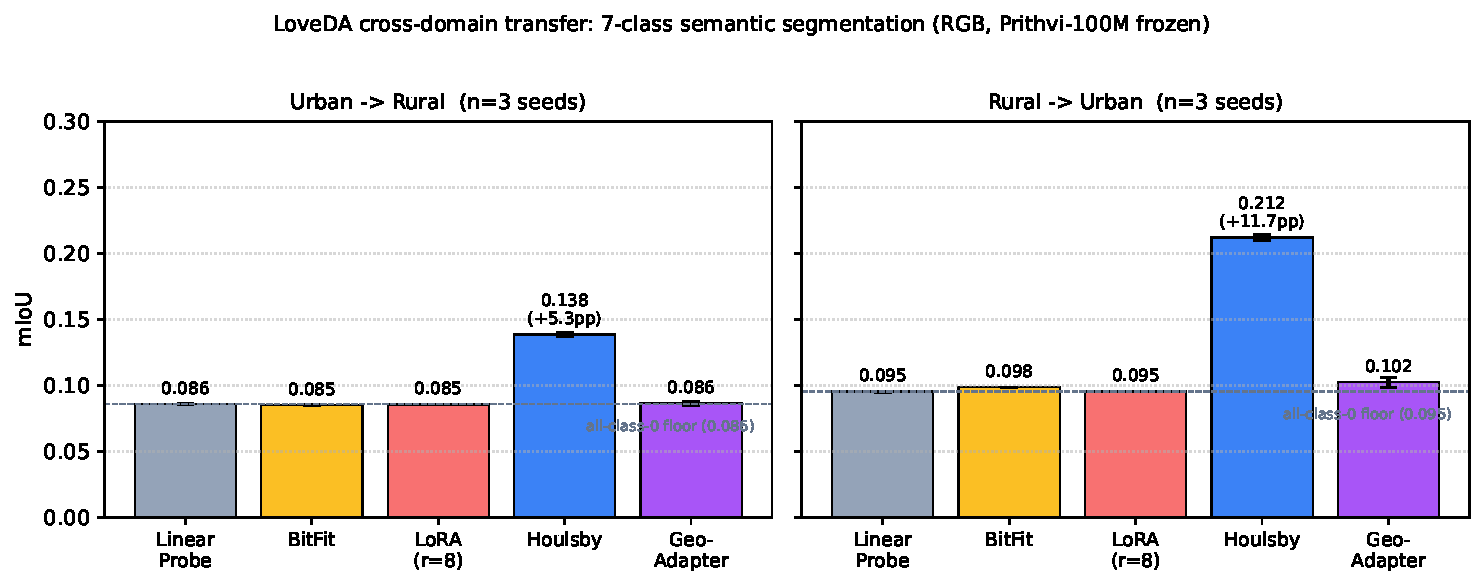
\includegraphics[width=0.95\linewidth]{figures/loveda_crossdomain.pdf}
\caption{LoveDA cross-domain transfer across five PEFT methods. Bars show mean mIoU over three seeds with standard-deviation error bars; the dashed line in each panel marks the all-class-0 majority-prediction floor (0.086 U$\rightarrow$R, 0.095 R$\rightarrow$U) computed from the validation class distribution. The Houlsby callout reports the absolute gain over the same-direction linear probe.}
\label{fig:loveda-cross}
\end{figure}

\paragraph{Full fine-tuning improves over the small-PEFT cluster but does not overtake Houlsby.} We additionally ran the Table~\ref{tab:loveda-cross} full fine-tuning baseline in both transfer directions. The U$\rightarrow$R seed values are 0.1119, 0.1142, and 0.1175; the R$\rightarrow$U seed values are 0.1481, 0.1381, and 0.1311. Both directions sit well above the small-PEFT cluster and the all-background floor, but they remain below Houlsby on the same directions. We therefore treat full fine-tuning as a stronger unfrozen baseline that narrows, but does not remove, the LoveDA cross-domain gap.

The cross-domain results add three findings to those reported on Linhe:

\paragraph{The Houlsby lead reproduces and grows under cross-domain stress.} Houlsby outperforms linear probing by $+0.0526$ mIoU under U$\rightarrow$R and $+0.1167$ mIoU under R$\rightarrow$U. The R$\rightarrow$U gap is the largest single-method advantage we observe in the entire paper. Linhe, three public benchmarks, and now LoveDA cross-domain all place Houlsby decisively ahead of every other PEFT method we test; we interpret this as the strongest evidence that the architecture-awareness recommendation in Section~\ref{sec:segmentation} is robust to label provenance, geographic split, and domain shift.

\paragraph{Small-PEFT methods cluster at the all-background baseline despite recovering a weak binary signal.} The four small-parameter methods --- linear probing (5.4k params), BitFit (128k), LoRA r=8 (153k), and GeoAdapter (5.5k) --- cluster within $\pm 0.001$ mIoU of one another in the U$\rightarrow$R direction at the 0.085--0.086 range, which lies within $1 \times 10^{-3}$ of the all-class-0 baseline (0.0858) computed by predicting only the dominant background class against the LoveDA validation class distribution. The same pattern holds R$\rightarrow$U at the 0.095--0.102 cluster. We instrument the streaming evaluator to record per-class IoU and the predicted-pixel histogram alongside aggregated mIoU. With 5$\times$ the LoRA learning rate and 2$\times$ the training budget (Appendix~\ref{app:loveda-perclass}), LoRA r=8 reaches mIoU $0.0901$ --- a +$0.0046$ gain over the protocol-default schedule --- but the per-class signature reveals that this gain is recovered almost entirely from a single binary distinction (background versus building, IoU $0.397$ and $0.201$ respectively) while five of the seven classes remain at zero IoU. Doubling the LoRA rank to 16 gives a statistically identical result. The cross-domain mIoU floor is therefore not pure majority-class collapse but a more constrained failure: small-capacity PEFT recovers a weak two-class discrimination whose signal is diluted to near-baseline levels by the seven-class macro average, and increasing the optimization budget by an order of magnitude does not push the recovered signature beyond binary.

\paragraph{A capacity threshold separates multi-class transfer from binary recovery.} Houlsby's 1.2M trainable parameters are the only configuration in our sweep that recovers non-degenerate IoU on more than two classes simultaneously under domain shift. BitFit at 128k parameters and LoRA r=8 at 153k --- both 7$\times$ to 9$\times$ larger than the linear probe --- behave statistically indistinguishably from linear probing, and the diagnostic sweep confirms that even at 5$\times$ lr$_{\mathrm{peft}}$ and double the training budget, LoRA's recovered signal does not extend beyond a single binary distinction (Appendix~\ref{app:loveda-perclass}). This is qualitatively different from the within-domain Linhe results (where BitFit was $+0.020$ and GeoAdapter $+0.087$ above linear probing); the cross-domain protocol appears to impose a per-method capacity threshold below which adapters cannot recover multi-class discriminative content from a frozen Prithvi backbone whose pretraining distribution does not include the LoveDA scene statistics. The threshold falls cleanly between LoRA r=16 ($\approx$$3 \times 10^5$ params, mIoU $0.0900$ at extended schedule) and Houlsby ($\approx$$1.2 \times 10^6$ params, mIoU $0.1384$ at default schedule). To our knowledge this is the first systematic per-method capacity-threshold report for PEFT on a public remote-sensing cross-domain benchmark, and it is actionable: a practitioner deploying a frozen geospatial foundation model on a target domain that drifts substantially from pretraining should budget on the order of $10^6$ trainable adapter parameters for full multi-class transfer, not the $10^5$ commonly reported as ``parameter-efficient'' on within-domain transfer.

\subsection{Discussion}

The Linhe results confirm that the Houlsby $\gg$ Linear~Probe ordering reported on three public benchmarks reproduces on a heterogeneous sub-meter Chinese-domestic RGB corpus with a geographic-split protocol. The LoveDA cross-domain replication strengthens the same ordering on a public benchmark explicitly designed to stress urban/rural transfer. Three observations are specific to the production / cross-domain setting and not visible in within-domain public benchmarks:

\begin{enumerate}[leftmargin=1.5em,itemsep=0.2em]
    \item \emph{The PEFT delta is mediated by label quality.} Synthetic weak labels yield a $+0.017$ mIoU PEFT delta on Linhe; production Esri labels yield $+0.116$. Method-only papers that report a single delta number on a single dataset risk misleading practitioners about the operating point they should expect.
    \item \emph{Geographic split changes the absolute numbers.} A patch-level random split on the same Linhe data and methods yields linear-probe mIoU of $0.244$ and Houlsby mIoU of $0.401$; the gap is preserved but both numbers are inflated relative to the scene-level split we report. Practitioners deploying these models on new scenes should expect numbers closer to the scene-level column.
    \item \emph{Domain shift imposes a per-method capacity threshold for multi-class transfer.} Section~\ref{sec:loveda} shows that under LoveDA cross-domain, every PEFT method below $\approx$$10^6$ trainable parameters fails to recover multi-class discriminative content; the diagnostic sweep in Appendix~\ref{app:loveda-perclass} shows that even at 10$\times$ the optimization budget, sub-$10^6$ adapters reach at most a single binary class distinction. This is not visible on within-domain benchmarks, where small-parameter methods like BitFit and GeoAdapter recover meaningful gains. Practitioners should budget adapter capacity by target-domain drift and label cardinality, not only by within-domain accuracy economy.
    \item \emph{Class imbalance is a property of the geography, not a defect.} Hetao agricultural land has near-zero forest cover. PEFT methods do not redistribute attention toward absent classes; honest reporting on real geography includes the empirical distribution rather than imposing a synthetic balance.
\end{enumerate}

This section therefore strengthens the central claim of the paper from ``the ranking is consistent across three public benchmarks'' to ``the ranking is consistent across three public benchmarks, one production GIS deployment, and a public cross-domain replication.'' The fused-QKV implementation trap, the input-stage failure mode of GeoAdapter, and the architecture-awareness recommendation in Section~\ref{sec:segmentation} all carry over without modification; we re-instantiate them on Linhe and on LoveDA for completeness in Appendices~\ref{app:linhe-perseed} and~\ref{app:loveda-perclass}.
